\documentclass[a4paper,12pt]{ctexart}
\usepackage{../../teaching-style}

\begin{document}
\pagestyle{empty}

\maintitle{几何 上册}
\begin{center}
  \large 低学段 · 三角形、四边形、相似与圆
\end{center}
\vspace{0.3cm}

\chaptertitle{第一章\quad 角度计算基础}

\sectiontitle{1.1\quad 角的概念与分类}

\knowbox{
角：从一点引出的两条射线所组成的图形。\\
角的分类：锐角($0^\circ<\alpha<90^\circ$)、直角($\alpha=90^\circ$)、钝角($90^\circ<\alpha<180^\circ$)、平角($180^\circ$)、周角($360^\circ$)。\\
余角：两角之和为$90^\circ$，互余。\\
补角：两角之和为$180^\circ$，互补。}

\sectiontitle{1.2\quad 对顶角与邻补角}

\knowbox{
对顶角相等。\\
邻补角互补。\\
两条直线相交，对顶角有两对，邻补角有四对。}

\sectiontitle{1.3\quad 平行线中的角}

\knowbox{
同位角相等，内错角相等，同旁内角互补$\Leftrightarrow$两直线平行。}

\begin{center}
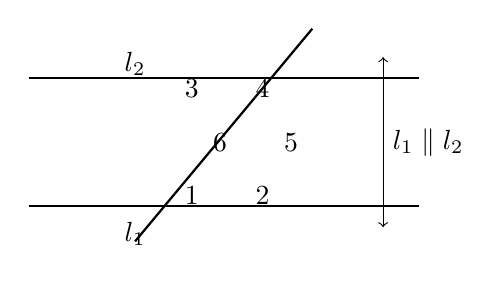
\begin{tikzpicture}[scale=0.9]
\draw[thick] (-0.5,0) -- (5,0);
\draw[thick] (-0.5,1.8) -- (5,1.8);
\draw[thick] (1,-0.5) -- (3.5,2.5);
\node at (1.8,0.15) {$1$};
\node at (2.8,0.15) {$2$};
\node at (1.8,1.65) {$3$};
\node at (2.8,1.65) {$4$};
\node at (3.2,0.9) {$5$};
\node at (2.2,0.9) {$6$};
\draw[<->] (4.5,-0.3) -- (4.5,2.1) node[midway,right] {$l_1\parallel l_2$};
\node at (1,-0.4) {$l_1$};
\node at (1,2) {$l_2$};
\end{tikzpicture}
\end{center}

\sectiontitle{习题1}

\begin{exercise}
\item $\angle A=35^\circ$，求它的余角和补角。
\item 两个角互为余角且相等，求这两个角的度数。
\item 如图所示（描述），直线$a\parallel b$，$\angle1=72^\circ$，求$\angle2$、$\angle3$、$\angle4$的度数。
\item 一个角的补角是这个角的$3$倍，求这个角的度数。
\end{exercise}

\newpage

\chaptertitle{第二章\quad 三角形}

\sectiontitle{2.1\quad 三角形的内角和与外角}

\knowbox{
三角形内角和$=180^\circ$。\\
外角等于不相邻的两个内角之和。\\
三角形的一个外角大于任何一个不相邻的内角。}

\sectiontitle{2.2\quad 三角形的分类}

\knowbox{
按角分：锐角三角形、直角三角形、钝角三角形。\\
按边分：不等边三角形、等腰三角形、等边三角形。\\
等腰三角形：两腰相等，两底角相等，"三线合一"。\\
等边三角形：三边相等，三个角都是$60^\circ$。}

\sectiontitle{2.3\quad 三边关系}

\knowbox{三角形任意两边之和大于第三边，任意两边之差小于第三边。}

\sectiontitle{2.4\quad 三角形的高、中线、角平分线}

\knowbox{
\textbf{高}：从顶点向对边作垂线。三条高交于一点（垂心）。\\
\textbf{中线}：连接顶点和对边中点。三条中线交于一点（重心），重心分中线$2:1$。\\
\textbf{角平分线}：平分内角的线。三条角平分线交于一点（内心，内切圆圆心）。}

\begin{center}
\begin{tikzpicture}[scale=0.9]
% 三角形
\coordinate (A) at (0,0);
\coordinate (B) at (4,0);
\coordinate (C) at (1.5,2.5);
\draw[thick] (A) -- (B) -- (C) -- cycle;
\node[below] at (A) {$A$};
\node[below] at (B) {$B$};
\node[above] at (C) {$C$};
% 高
\draw[dashed] (C) -- (1.5,0) node[below] {$D$};
\draw (1.5,0.15) -- (1.65,0.15) -- (1.65,0);
% 中线
\coordinate (M) at (2,0);
\draw[dotted, thick] (C) -- (M) node[below] {$M$};
% 角平分线
\draw[dashdotted] (A) -- (2.3,1.2) node[above,yshift=0.2cm] {$AD$平分$\angle A$};
\draw (0.8,0.4) arc (30:60:0.5);
\draw (0.95,0.55) arc (20:40:0.7);
\node at (3,1.2) {高$CF$};
\node at (3.2,0.5) {中线$CM$};
\end{tikzpicture}
\end{center}

\sectiontitle{习题2}

\begin{exercise}
\item 一个三角形中，$\angle A=50^\circ$，$\angle B=65^\circ$，求$\angle C$。
\item 等腰三角形的一个底角为$40^\circ$，求顶角的度数。
\item 等腰三角形的一条边长为$5$，另一条边长为$8$，求周长。
\item 等腰三角形的一个角为$100^\circ$，求另外两个角的度数。
\item 直角三角形中，两个锐角的度数比为$2:3$，求这两个锐角的度数。
\end{exercise}

\newpage

\chaptertitle{第三章\quad 全等三角形}

\sectiontitle{3.1\quad 全等三角形的判定}

\knowbox{
\textbf{SSS}：三边对应相等。\\
\textbf{SAS}：两边及夹角对应相等。\\
\textbf{ASA}：两角及夹边对应相等。\\
\textbf{AAS}：两角及其中一角的对边对应相等。\\
\textbf{HL}（直角三角形）：斜边和一条直角边对应相等。}

\sectiontitle{3.2\quad 全等三角形的性质}

\knowbox{对应边相等，对应角相等，对应线段（中线、高、角平分线）相等。}

\sectiontitle{习题3}

\begin{exercise}
\item 已知$\triangle ABC\cong\triangle DEF$，$\angle A=50^\circ$，$\angle B=70^\circ$，$AB=5$，求$\angle D$、$\angle F$和$DE$的长。

\item 如图（描述），$AB=AD$，$\angle BAC=\angle DAC$，求证：$\triangle ABC\cong\triangle ADC$。

\item 如图，$AB=CD$，$AB\parallel CD$，求证：$\triangle ABD\cong\triangle CDB$。

\item 如图，$AC\perp BC$，$AD\perp BD$，$AC=BD$，求证：$BC=AD$。

\item 如图，$AB=AC$，$DB=DC$，求证：$\angle B=\angle C$。
\end{exercise}

\newpage

\chaptertitle{第四章\quad 四边形}

\sectiontitle{4.1\quad 平行四边形}

\knowbox{
定义：两组对边分别平行的四边形。\\
性质：对边平行且相等，对角相等，邻角互补，对角线互相平分。\\
判定：两组对边分别平行$\big/$相等；一组对边平行且相等；对角线互相平分。}

\sectiontitle{4.2\quad 特殊平行四边形}

\knowbox{
\textbf{矩形}：有一个角是直角的平行四边形。对角线相等。\\
\textbf{菱形}：有一组邻边相等的平行四边形。对角线垂直平分，平分内角。\\
\textbf{正方形}：既是矩形又是菱形。对角线相等且垂直平分。}

\sectiontitle{4.3\quad 多边形内角和}

\knowbox{$n$边形内角和$=(n-2)\times180^\circ$，外角和$=360^\circ$。}

\sectiontitle{习题4}

\begin{exercise}
\item 平行四边形$ABCD$中，$\angle A=120^\circ$，求另外三个角的度数。
\item 矩形的一条对角线长为$10$，一条边长为$6$，求另一条边长和面积。
\item 菱形边长为$5$，一条对角线长为$6$，求另一条对角线的长。
\item 求证：正方形的对角线相等且互相垂直平分。
\item 一个多边形的内角和是$1080^\circ$，它是几边形？
\end{exercise}

\newpage

\chaptertitle{第五章\quad 相似三角形}

\sectiontitle{5.1\quad 比例线段与平行线分线段成比例}

\knowbox{
平行线分线段成比例定理：三条平行线截两条直线，所得对应线段成比例。\\
平行于三角形一边的直线截其他两边，所得对应线段成比例。}

\sectiontitle{5.2\quad 相似三角形的判定}

\knowbox{
\textbf{AA}：两角对应相等，两三角形相似。\\
\textbf{SAS}：两边对应成比例且夹角相等。\\
\textbf{SSS}：三边对应成比例。\\
平行于三角形一边的直线与其他两边相交，所截三角形与原三角形相似。}

\sectiontitle{5.3\quad 相似三角形的性质}

\knowbox{
相似三角形对应角相等，对应边成比例。\\
对应高的比$=$对应中线的比$=$对应角平分线的比$=$对应周长的比$=$相似比。\\
面积比$=$相似比的平方。}

\sectiontitle{习题5}

\begin{exercise}
\item $\triangle ABC\sim\triangle DEF$，相似比为$2:3$。若$AB=6$，求$DE$。

\item 如图，$DE\parallel BC$，$AD=3$，$DB=2$，$AE=4.5$，求$EC$和$AC$。

\item 两个相似三角形的面积比为$16:25$，求它们的周长比。

\item 如图，$\angle1=\angle2$，$AB=6$，$AC=9$，$AD=4$，求证：$\triangle ABC\sim\triangle AED$。

\item 在同一时刻，一根$1.5$米高的竹竿影长为$1$米，一座楼的影长为$10$米，求楼高。
\end{exercise}

\newpage

\chaptertitle{第六章\quad 圆}

\sectiontitle{6.1\quad 圆的基本概念}

\knowbox{
圆：到定点（圆心）距离等于定长（半径）的点的集合。\\
弦：连接圆上任意两点的线段。直径是最长的弦。\\
弧：圆上任意两点间的部分。\\
圆心角：顶点在圆心的角。\\
圆周角：顶点在圆上，两边与圆相交的角。}

\sectiontitle{6.2\quad 垂径定理}

\knowbox{垂直于弦的直径平分弦，并且平分弦所对的两条弧。\\
平分弦（不是直径）的直径垂直于弦，并且平分弦所对的两条弧。}

\begin{center}
\begin{tikzpicture}[scale=0.8]
\draw[thick] (0,0) circle (2.5);
\draw[thick] (-2.5,0) -- (2.5,0);
\draw[thick] (-1.5,-1.8) -- (1.5,-1.2);
\draw[dashed] (0,0) -- (0,-2.5);
\filldraw (0,0) circle (1.5pt) node[above right] {$O$};
\filldraw (0,-2.5) circle (1.5pt) node[below] {$D$};
\filldraw (1.5,-1.2) circle (1.5pt) node[right] {$B$};
\filldraw (-1.5,-1.8) circle (1.5pt) node[left] {$A$};
\filldraw (0,-1.5) circle (1.5pt) node[right] {$C$};
\draw (0.3,-1.5) -- (0.3,-1.2) -- (0,-1.2);
\node at (2.2,0.3) {直径$CD$};
\node at (2.2,-1.5) {弦$AB$};
\node at (0,-0.8) {$CD\perp AB$};
\node at (0.8,-2.2) {$AC=BC$};
\end{tikzpicture}
\end{center}

\sectiontitle{6.3\quad 圆周角定理}

\knowbox{
同弧所对的圆周角等于圆心角的一半。\\
直径所对的圆周角是直角（$90^\circ$）。\\
同弧所对的圆周角相等。}

\sectiontitle{6.4\quad 切线的判定与性质}

\knowbox{
判定：经过半径外端且垂直于半径的直线是圆的切线。\\
性质：圆的切线垂直于过切点的半径。\\
切线长定理：从圆外一点引圆的两条切线，切线长相等。}

\begin{center}
\begin{tikzpicture}[scale=0.8]
\draw[thick] (0,0) circle (2);
\draw[thick] (-1,2.5) -- (4,2.5);
\filldraw (0,0) circle (1.5pt) node[below] {$O$};
\filldraw (2,0) circle (1.5pt) node[right] {$A$};
\draw[thick] (0,0) -- (2,0);
\node at (1,-0.4) {$r$};
\draw (2,0.15) -- (1.85,0.15) -- (1.85,0);
\node at (3,2.2) {$l\perp OA$于$A$};
\node at (3,1.7) {$l$为切线};
% 切线长定理
\filldraw (-2,0) circle (1.5pt) node[below] {$P$};
\draw[thick] (-2,0) -- (-0.6,1.2);
\draw[thick] (-2,0) -- (0.6,1.2);
\filldraw (-0.6,1.2) circle (1.5pt) node[left] {$B$};
\filldraw (0.6,1.2) circle (1.5pt) node[right] {$C$};
\node at (-1.8,0.8) {$PB=PC$};
\end{tikzpicture}
\end{center}

\sectiontitle{6.5\quad 弧长与扇形面积}

\knowbox{
弧长$l=\dfrac{n\pi r}{180}$，扇形面积$S=\dfrac{n\pi r^2}{360}=\dfrac12 l r$。}

\sectiontitle{习题6}

\begin{exercise}
\item 已知圆的半径为$5$，一条弦长为$8$，求圆心到弦的距离。
\item 如图，$AB$是直径，$\angle ABC=30^\circ$，求$\angle BAC$。
\item 圆的半径为$6$，$60^\circ$圆心角所对的弧长和扇形面积。
\item 如图，$PA$、$PB$是$\odot O$的切线，$A$、$B$为切点，$\angle APB=50^\circ$，求$\angle AOB$。
\item 半径为$4$，弧长为$2\pi$的弧所对的圆心角是多少度？
\end{exercise}

\end{document}
